% NOTE:
% latexmk -shell-escape -pvc slides # This compiles a PDF after any changes.
% latexmk -c slides.tex             # This cleans temporal files.

\documentclass[aspectratio=169]{beamer}

\setbeamertemplate{footline}[frame number]
\beamertemplatenavigationsymbolsempty

% NOTE: User numeric style for references.
\usepackage[backend=biber, style=numeric]{biblatex}
\usepackage{caption}
\usepackage{graphicx}
\usepackage{hyperref}
\usepackage{subcaption}

\usetheme{Boadilla}
\usecolortheme{default}

\addbibresource{treeslab_workshop.bib}

\captionsetup[figure]{labelformat=empty}

\hypersetup{
    colorlinks,
    allcolors=.,
    urlcolor=blue,
  }

\title[References \& data]{Writing papers: references and data management}
\subtitle{The TREESLab way for reference management \& manuscripts' data curation}

\author[A. Sánchez]{
    Alber Ipia\inst{1} \\
    \href{mailto:alber.ipia@inpe.br}{alber.ipia@inpe.br}
  }

\institute[INPE]{
  
\includegraphics[scale=0.5]{logos/trees-color-h_2.png} \\
  \inst{1} National Institute for Space Research
}

\date{\today}

\includeonly{
    tex/01_introduction,
    tex/02_reference_management,
    tex/03_data_management,
    tex/99_remarks,
  }

\setcounter{tocdepth}{2}

\begin{document}

\frame{\titlepage}

\begin{frame}[allowframebreaks]
  \frametitle{Agenda} \tableofcontents
\end{frame}

\section{Introduction}

\begin{frame}
  What do researchers do?
\end{frame}

\begin{frame}
  \frametitle{Use, make, and share open results}
  \begin{figure}
    \centering
    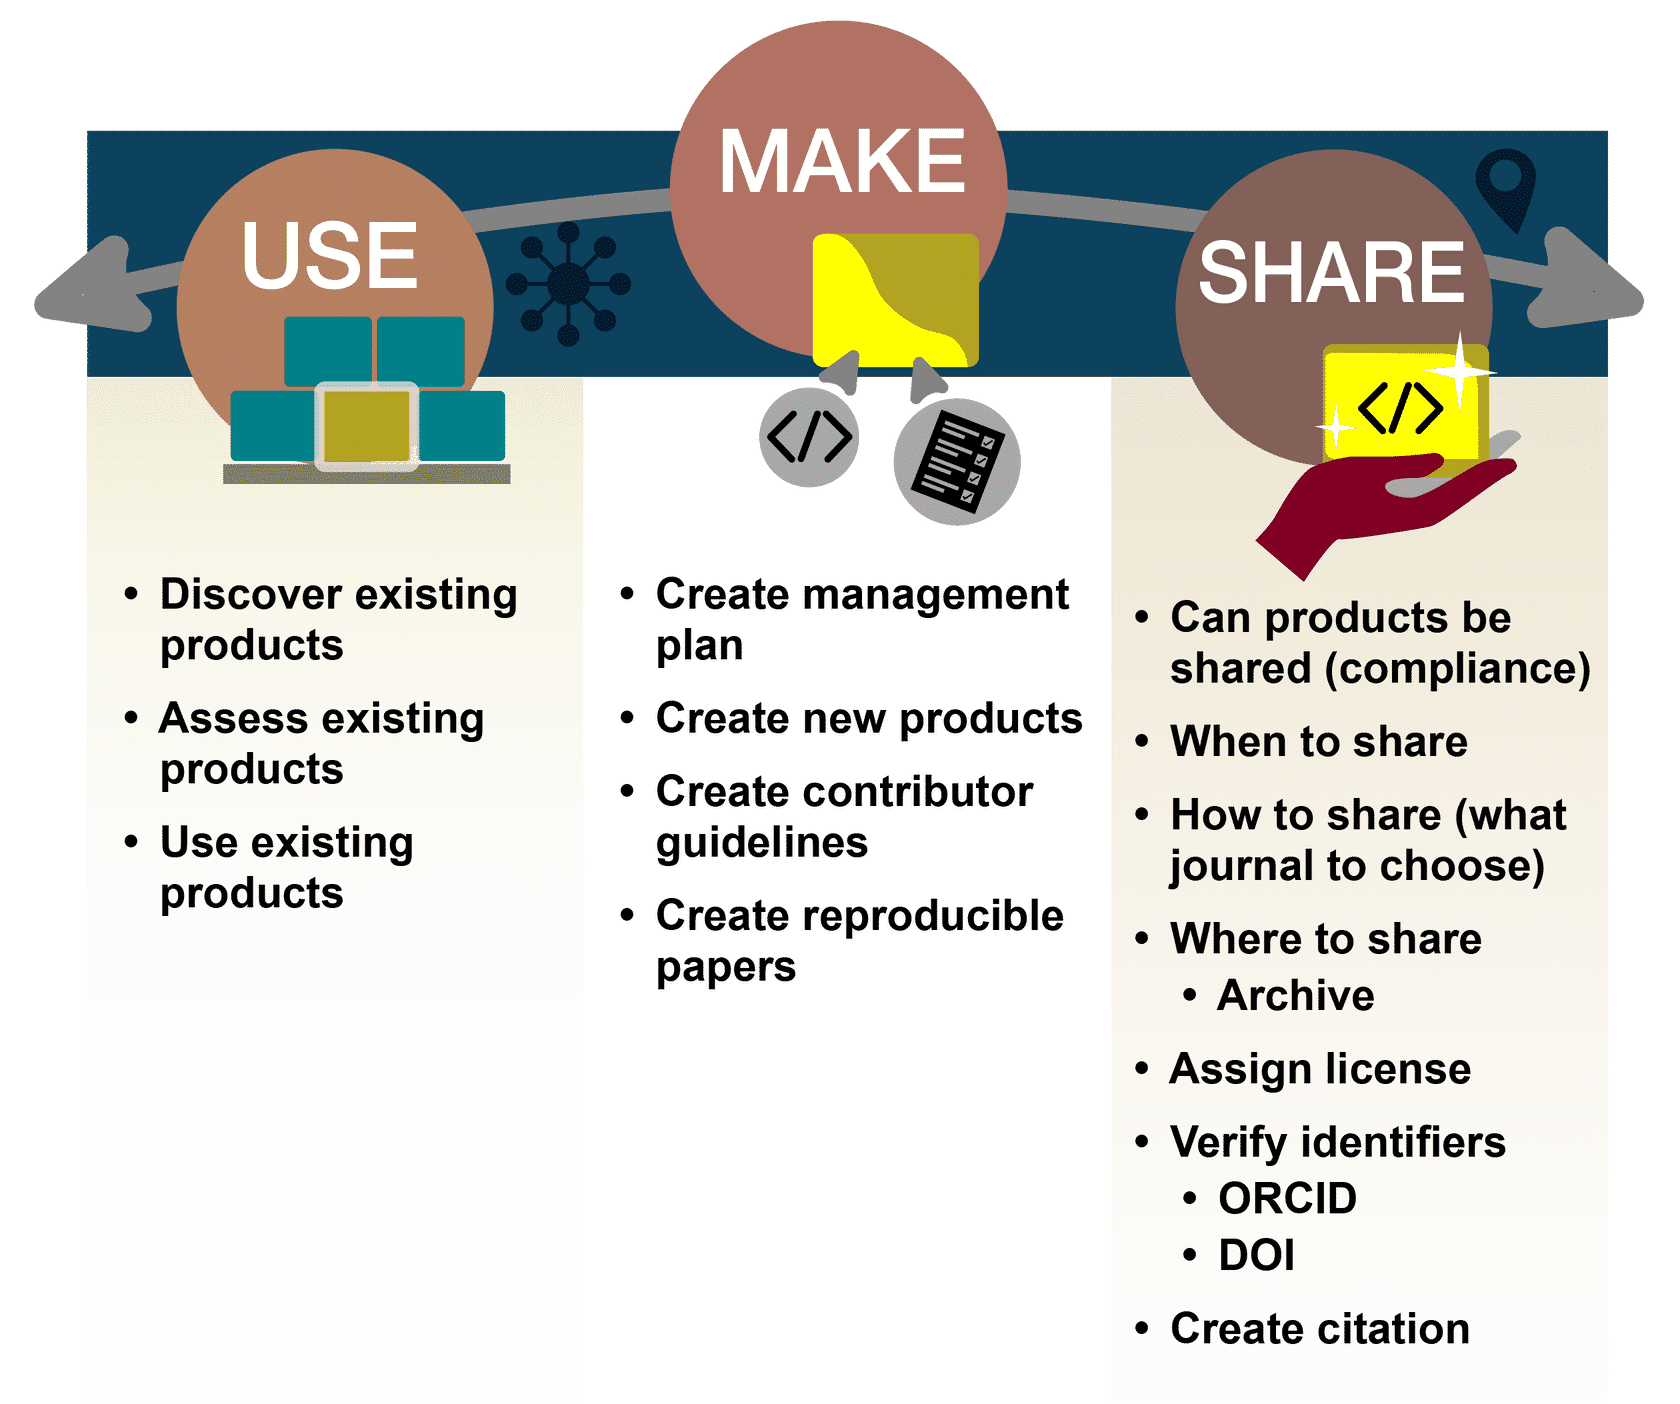
\includegraphics[width=0.5\textwidth]{images/use_make_share.png}
    \label{fig:use_make_share}
    \caption{
Source: \href{https://stemgateway.nasa.gov/s/course-offering/a0BSJ0000049ih3/open-science-101
    }
    {OpenScience101.org}}
  \end{figure}
\end{frame}

\begin{frame}
  \frametitle{The research cycle}
  \begin{figure}
    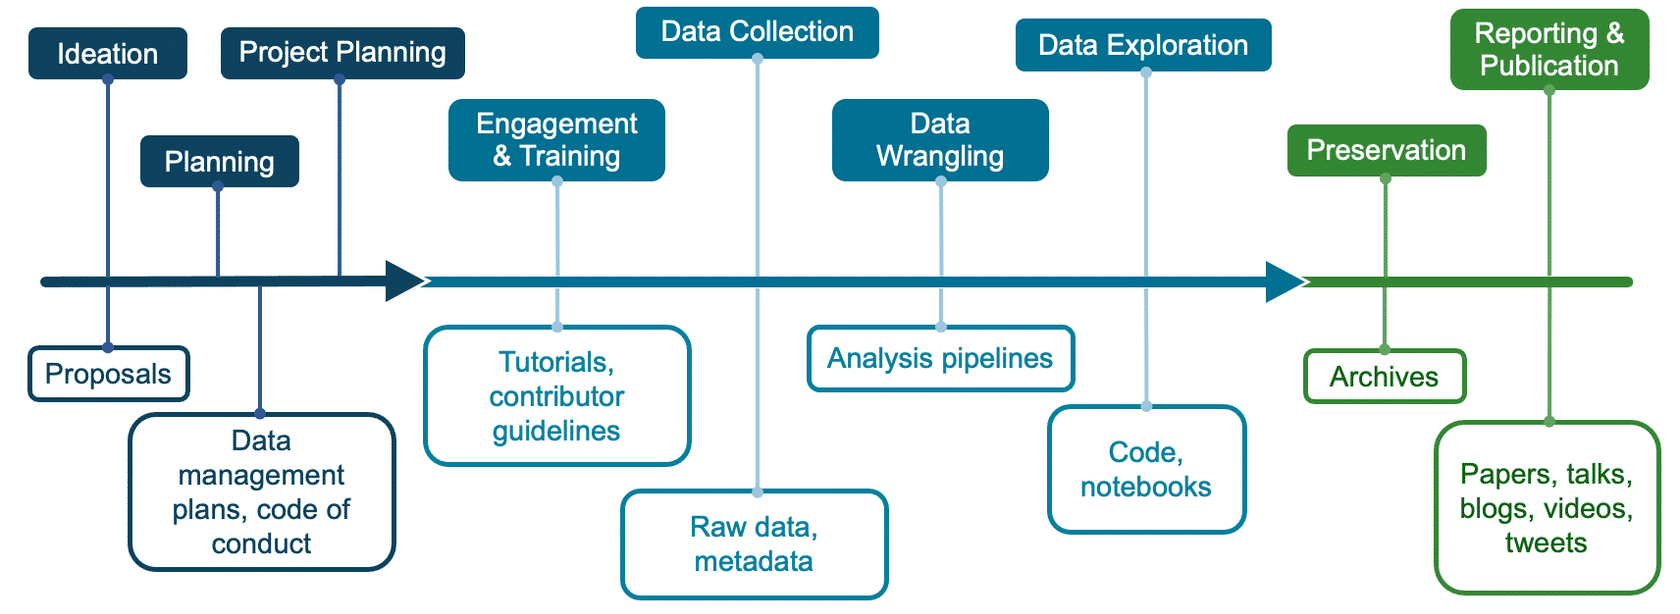
\includegraphics[width=0.9\textwidth]{images/research_cycle.png}
    \label{fig:research_cycle}
    \caption{
Source: \href{https://stemgateway.nasa.gov/s/course-offering/a0BSJ0000049ih3/open-science-101
    }
    {OpenScience101.org}}
  \end{figure}
\end{frame}

\begin{frame}
  \frametitle{Introduction}
  \begin{itemize}
    \item The scientific endeavour is time-consuming.
    \item Scientific research includes, among other tasks, keep track of the
    current scientific literature and use to foster new discoveries.
    \item But also, ensuring the scientific reproducibility of their
    experiments.
    \item Some work related to these task could done using specialized
    software and tools.
  \end{itemize}
\end{frame}

\begin{frame}
  \frametitle{Digital Object Identifier DOI}
  \begin{columns}
    \begin{column}{0.5\textwidth}
      \begin{itemize}
        \item Unique.
        \item Identifier.
        \item Persistent.
        \item Resolvable.
        \item Metadata.
        \item FAIR:
          \begin{itemize}
            \item Findable.
            \item Accessible.
            \item Interoperable.
            \item Reusable.
          \end{itemize}
      \end{itemize}
    \end{column}
    \begin{column}{0.5\textwidth}
      \begin{figure}
        \centering
        
\includegraphics[scale=0.7]{logos/doi_logo.png}
      \end{figure}
    \end{column}
  \end{columns}
\end{frame}

\section{Reference management}

\begin{frame}
  Reference management.
\end{frame}

\subsection{Reference management software}

\begin{frame}
  \frametitle{Reference management}
    \begin{columns}
      \begin{column}{0.5\textwidth}
        What do researches do with bibliographic
        references?~\cite{rongilmour2011}
        \begin{itemize}
          \item Import them from databases.
          \item Organize them.
          \item Gather additional metadata.
          \item Highlight and add notes to them.
          \item Sharing them.
          \item Convert them between formats or styles.
          \item Insert them to documents using word processing software.
        \end{itemize}
      \end{column}
      \begin{column}{0.5\textwidth}
        \begin{figure}
          \centering
          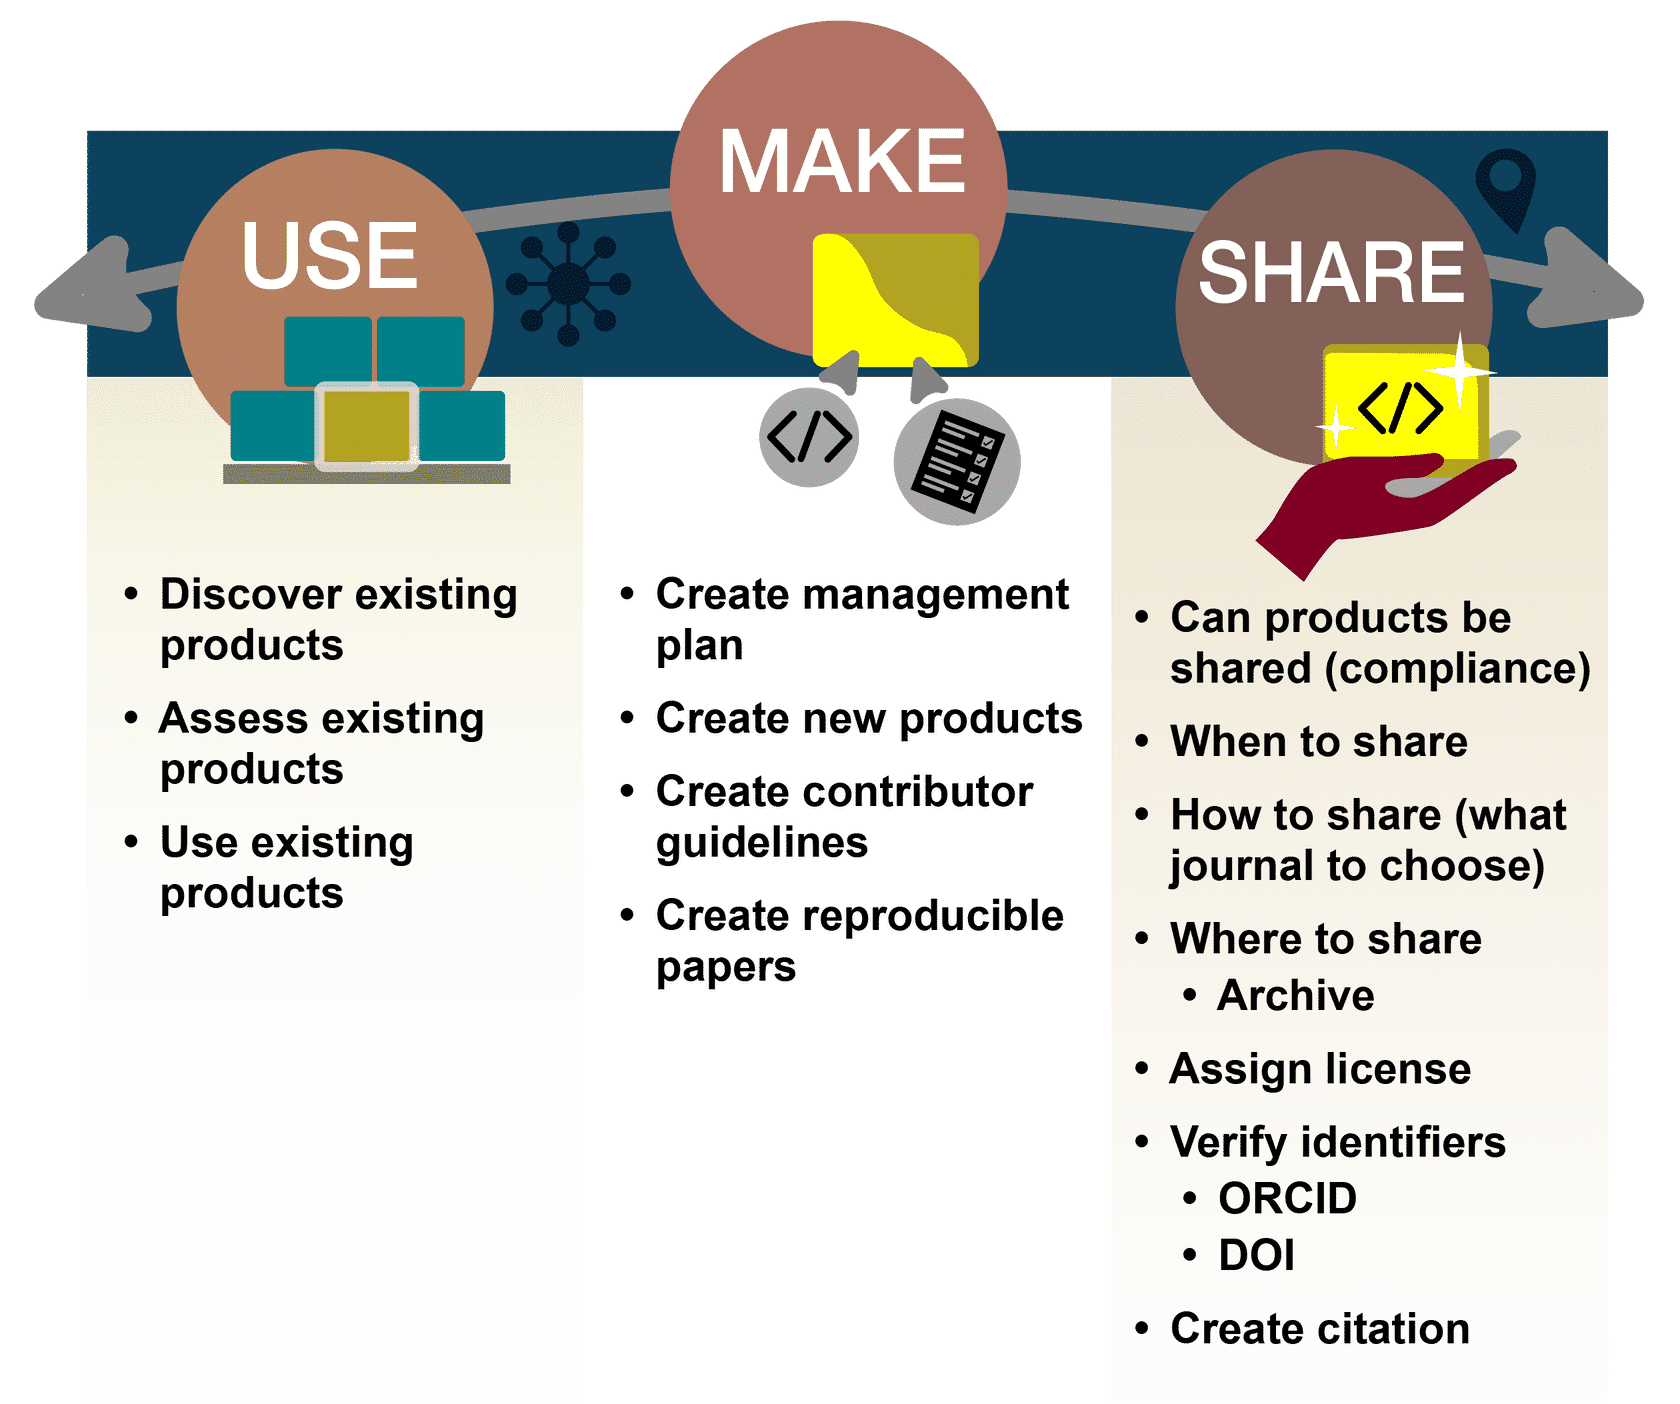
\includegraphics[width=0.97\textwidth]{images/use_make_share.png}
          \label{fig:use_make_share}
          \caption{
            Source:
            \href{https://stemgateway.nasa.gov/s/course-offering/a0BSJ0000049ih3/open-science-101}{OpenScience101.org}
            ~\cite{nasatopsopenscience101}.
          }
        \end{figure}
      \end{column}
    \end{columns}
\end{frame}

\begin{frame}[label={tools-reference-management}]
  \frametitle{Tools for reference management}  
      \begin{columns}
        \begin{column}{0.5\textwidth}
      \begin{itemize}
        \item There are at least 15 pieces of software for reference management.
        \item \citeauthor{rongilmour2011} made a comparison between
          CiteULike, RefWorks, Mendeley, and Zotero~\cite{rongilmour2011} in
          2011.
        \item For a more up-to-date comparison, also check
          \href{https://en.wikipedia.org/wiki/Comparison_of_reference_management_software}
          {software comparison article in Wikipedia.}
      \end{itemize}
    \end{column}
    \begin{column}{0.5\textwidth}
      \begin{figure}
        \centering
        
\includegraphics[scale=0.3]{images/RTFM_coffee_mug.jpg}
        \caption{Google is your friend. Source:~
          \href{https://en.wikipedia.org/w/index.php?title=Google_is_your_friend&redirect=no}
          {Wikipedia}}
      \end{figure}
    \end{column}
  \end{columns}
\end{frame}

\subsection{Zotero}

\begin{frame}
  \frametitle{Zotero}
  \begin{columns}
    \begin{column}{0.5\textwidth}
      \begin{itemize}
        \item Free and open source reference management software
        (AGPL v3 license).
        \item Free cloud storage up to 300 MB. 
        \item Released in 2006.
        \item Commonly used in medicine~\cite{mueenahmed2011,vanhecke2008}.
        \item Integration with Word Processor Software (MS Word, LibreOffice
          Writer, OnlyOffice, and Google docs).
        \item Integration with Web Browsers (Firefox, Chrome, Safari, Edge).
      \item Download \href{https://www.zotero.org/download/}{here}.
      \end{itemize}
    \end{column}
    \begin{column}{0.5\textwidth}
      \begin{figure}
        \centering
        
\includegraphics[scale=0.7]{logos/logo_zotero.png}
      \end{figure}
    \end{column}
  \end{columns}
\end{frame}

\begin{frame}
  \frametitle{Import references to Zotero}
  \begin{columns}
    \begin{column}{0.5\textwidth}
      Import references from other software:
      \begin{itemize}
        \item Mendeley.
        \item EndNote.
        \item Citavi.
        \item MS Word bibliography XML.
        \item Plain text.
        \item Bib(La)Tex.
        \item JabRef.
        \item Check how
          \href{https://www.zotero.org/support/moving_to_zotero}{here}.
      \end{itemize}
    \end{column}
    \begin{column}{0.5\textwidth}
      \begin{figure}
        \centering
        
\includegraphics[scale=0.4]{logos/citavi-all-logo-300x106.png}
        
\includegraphics[scale=0.25]{logos/EndNote.png}
        
\includegraphics[scale=0.3]{logos/Mendeley.png}
        
\includegraphics[scale=0.02]{logos/Microsoft-Word-Symbol.png}
      \end{figure}
    \end{column}
  \end{columns}
\end{frame}

\begin{frame}
  \frametitle{Organize references into collections}
  \begin{columns}
    \begin{column}{0.5\textwidth}
      \begin{itemize}
        \item References can be organized into collections.
        \item Collections allow hierarchical organization.
        \item The same item (reference) can belong to multiple collections.
        \item Use drag and drop to add items to collections.
        \item The TREESLab library has a collection for each project.
      \end{itemize}
    \end{column}
    \begin{column}{0.5\textwidth}
      \begin{figure}
        \centering
        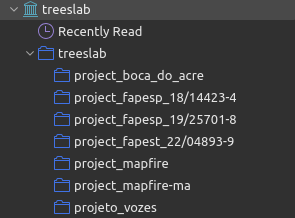
\includegraphics[scale=0.6]{images/treeslab_zotero_collections.png}
      \end{figure}
    \end{column}
  \end{columns}
\end{frame}

\begin{frame}
  \frametitle{Gather additional metadata}
  \begin{columns}
    \begin{column}{0.5\textwidth}
      \begin{itemize}
        \item Zotero allows you to fill additional metadata for each item.
        \item You can even associate a PDF to an item (reference) in Zotero.
      \end{itemize}
    \end{column}
    \begin{column}{0.5\textwidth}
      \begin{figure}
        \centering
        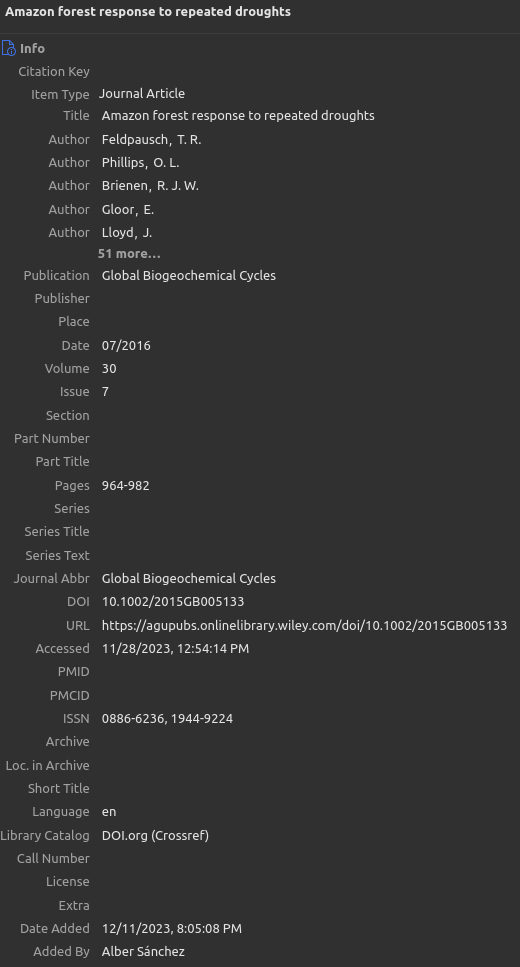
\includegraphics[scale=0.20]{images/treeslab_example.png}
      \end{figure}
    \end{column}
  \end{columns}
\end{frame}

\begin{frame}
  \frametitle{Highlight and add notes to references}
  \begin{columns}
    \begin{column}{0.5\textwidth}
      \begin{itemize}
        \item Zotero allows you to highlight and add notes to a PDF associated
          to an item (reference).
        \item You can also add notes to your highlights, to a (help \href{https://www.zotero.org/support/notes}{here}).
      \end{itemize}
    \end{column}
    \begin{column}{0.5\textwidth}
      \begin{figure}
        \centering
        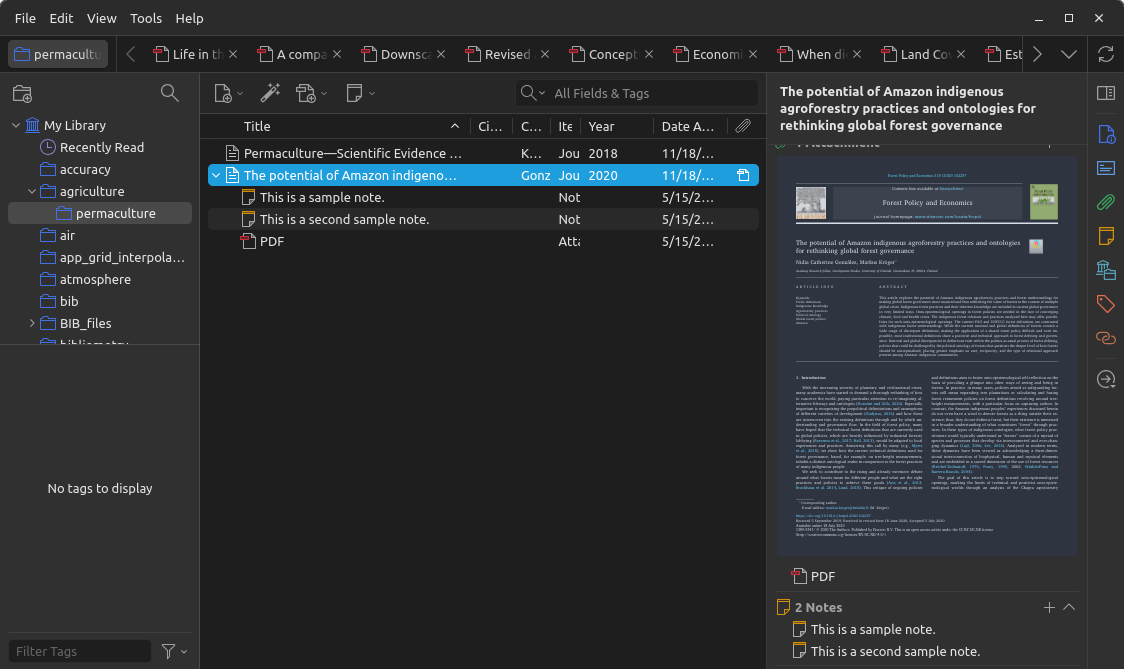
\includegraphics[scale=0.19]{images/zotero_pdf_notes.png}
      \end{figure}
    \end{column}
  \end{columns}
\end{frame}

\begin{frame}
  \frametitle{Share references}
  \begin{columns}
    \begin{column}{0.5\textwidth}
      \begin{itemize}
        \item Zotero allows you to create groups and use them to share references
          with colleagues.
        \item The TREESLab' publication list is a collection associated with the
          Zotero group called \textit{treeslab}.
      \end{itemize}
    \end{column}
    \begin{column}{0.5\textwidth}
      \begin{figure}
        \centering
        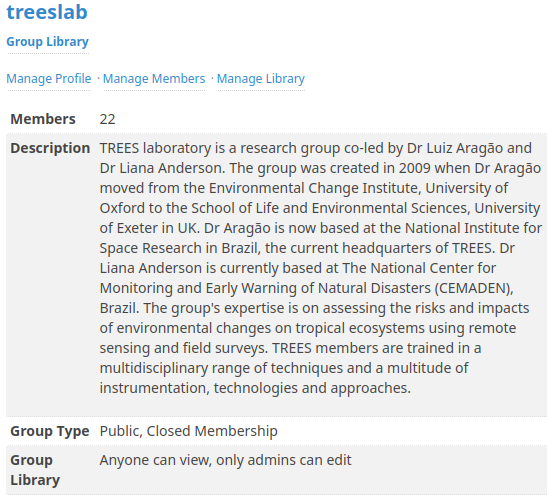
\includegraphics[scale=0.35]{images/treeslab_zotero_group.png}
      \end{figure}
    \end{column}
  \end{columns}
\end{frame}

\begin{frame}[label={convert_styles}]
  \frametitle{Convert references between formats or styles}
  \begin{columns}
    \begin{column}{0.5\textwidth}
      \begin{itemize}
        \item Zotero allows you to export items (references) or collections
          to several formats.
        \item It also allows to copy references and format them according
          to several reference styles.
        \item It is possible to add the ABTN style from
          \href{https://www.zotero.org/styles?q=abnt}{here}.
      \end{itemize}
    \end{column}
    \begin{column}{0.5\textwidth}
      \begin{figure}
        \centering
        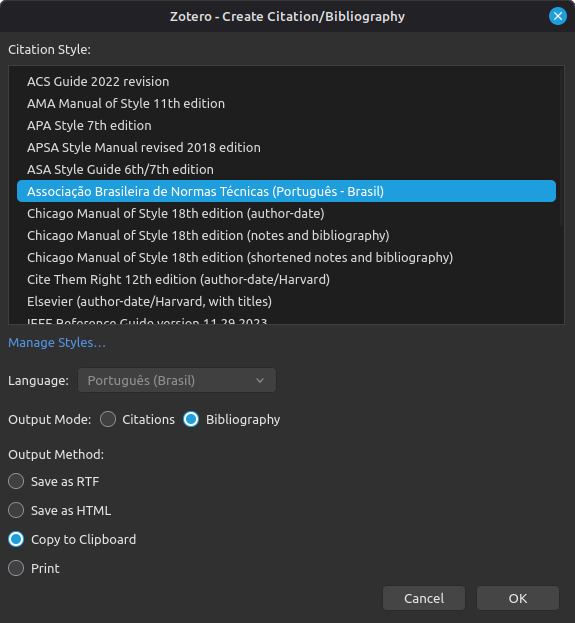
\includegraphics[scale=0.25]{images/zotero_citation_styles.png}
      \end{figure}
    \end{column}
  \end{columns}
\end{frame}

\begin{frame}
  \frametitle{Insert references into text documents}
  \begin{columns}
    \begin{column}{0.5\textwidth}
      \begin{itemize}
        \item \href{https://www.zotero.org/support/google_docs}{Google Docs} (using
          the Zotero connector for Web Browsers).
        \item \href{https://www.zotero.org/support/libreoffice_writer_plugin_usage}
          {Libre Office}.
        \item LaTeX (export collection to a BIB file).
        \item \href{https://www.zotero.org/support/word_processor_plugin_usage}
          {MS Word}.
      \end{itemize}
    \end{column}
    \begin{column}{0.5\textwidth}
      \begin{figure}
        
\includegraphics[scale=0.5]{logos/libreoffice-tdf-logo.png} \\
        \vspace{0.9cm}
        
\includegraphics[scale=0.3]{logos/Latex-Logo-Vector.png}
      \end{figure}
    \end{column}
  \end{columns}
\end{frame}

\begin{frame}[label=google_docs_zotero]
  \frametitle{Google Docs and Zotero}
  \begin{columns}
    \begin{column}{0.5\textwidth}
      \begin{itemize}
        \item Download the connector from
          \href{https://www.zotero.org/download/}{here}.
        \item Grant Google access to your Zotero account.
        \item Choose a style for your references.
        \item The Zotero menu in the tool bar is activated.
        \item Make sure your Zotero desktop instance is running.
        \item Add references to your text.
        \item Add a bibliography section.
      \end{itemize}
    \end{column}
    \begin{column}{0.5\textwidth}
      \begin{figure}
        \centering
        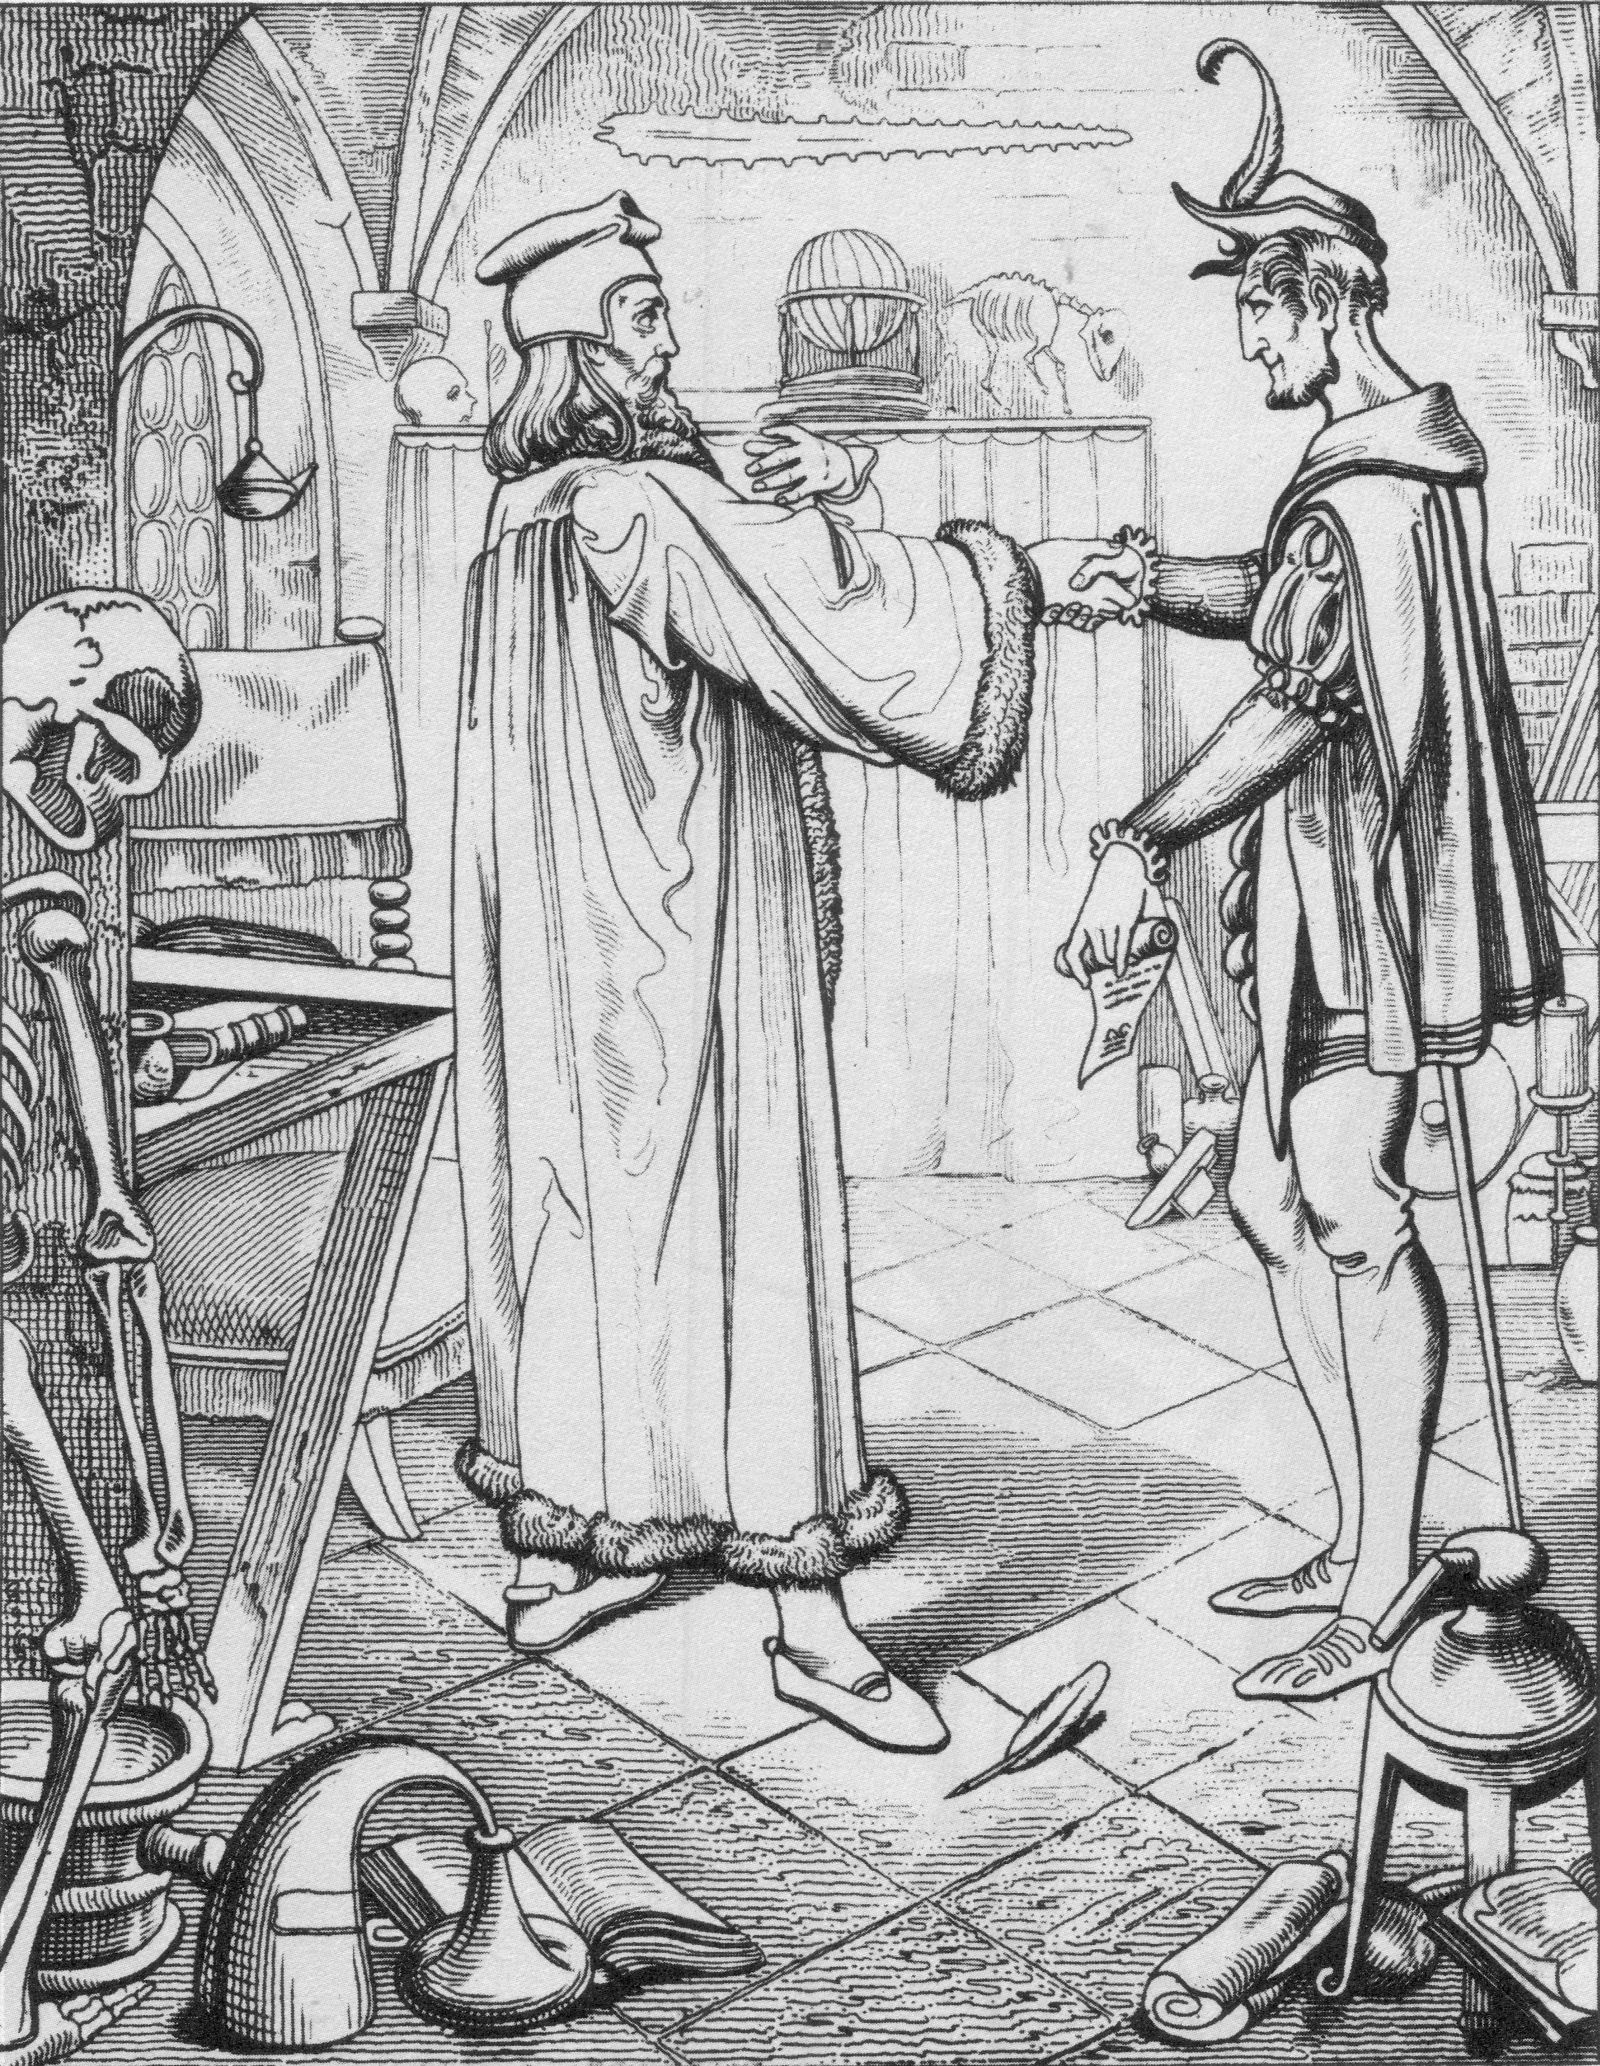
\includegraphics[scale=0.7]
        {images/Teufelspakt_Faust-Mephisto,_Julius_Nisle.jpg}
        \caption{Faustian bargain.
        Source:~\href{https://en.wikipedia.org/wiki/Deal_with_the_Devil}
        {Wikipedia}}
      \end{figure}
    \end{column}
  \end{columns}
\end{frame}

\subsection{Zotero and TREESLab}

\begin{frame}
  \frametitle{TREESLab group at Zotero}
  \begin{columns}
    \begin{column}{0.5\textwidth}
      \begin{itemize}
        \item TREESLab has a Zotero group (click
          \href{https://www.zotero.org/groups/5304570/treeslab}{here}).
        \item This group hosts TREESLab's publication list.
        \item The group owner is TREESLab's email account
          \href{mailto:wertreeslab@gmail.com}{wertreeslab@gmail.com}
        \item Here we keep track of the publications produced by TREESLab.
        \item TREESLab members don't have to be members to add their
          publications to the list (but it'd be nice, though).
      \end{itemize}
    \end{column}
    \begin{column}{0.5\textwidth}
      \begin{figure}
        \centering
        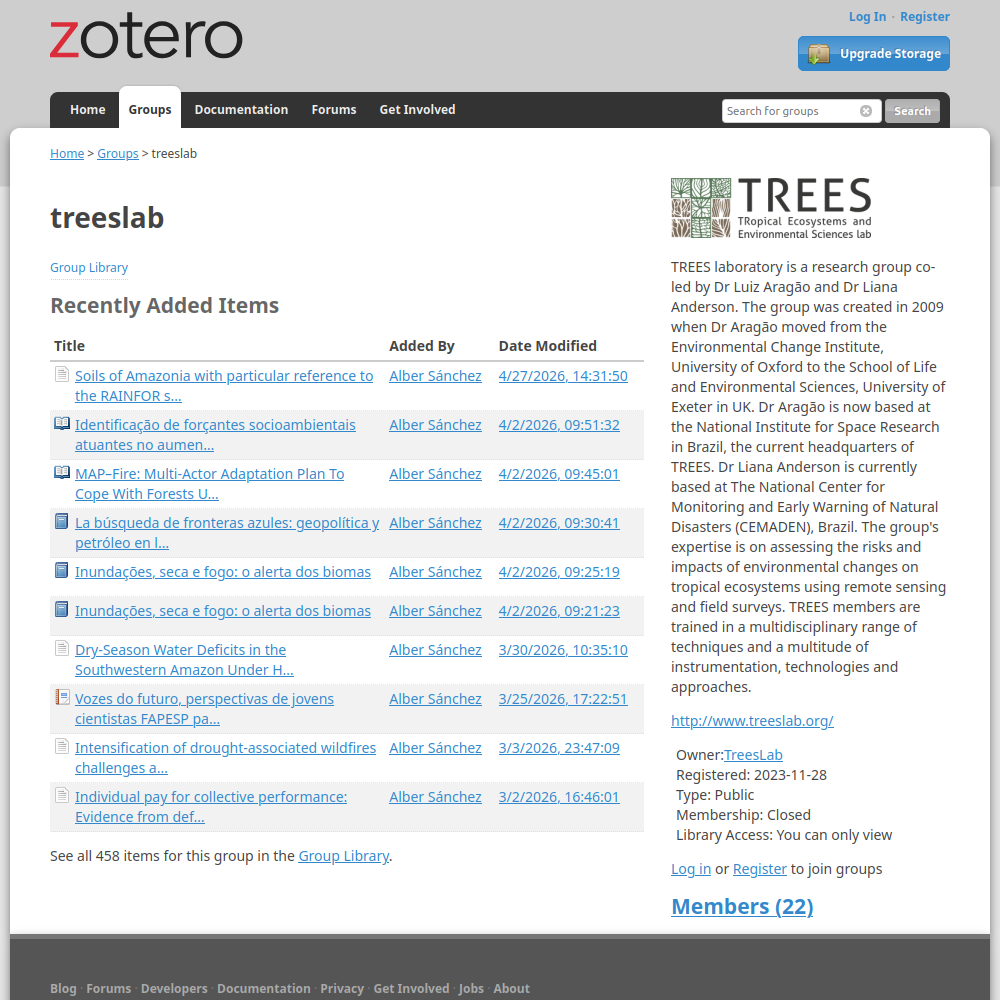
\includegraphics[scale=0.20]{images/zotero_group_treeslab.png}
      \end{figure}
    \end{column}
  \end{columns}
\end{frame}

\begin{frame}
  \frametitle{Researcher's profile at \url{zotero.org}}
  \begin{columns}
    \begin{column}{0.5\textwidth}
      \begin{itemize}
        \item Researchers can build a profile and \url{zotero.org} will host it.
        \item This profile would display the items in the
          \textit{My Publicatons} collection (check \href{https://www.zotero.org/support/my_publications}{here}).
      \end{itemize}
    \end{column}
    \begin{column}{0.5\textwidth}
      \begin{figure}
        \centering
        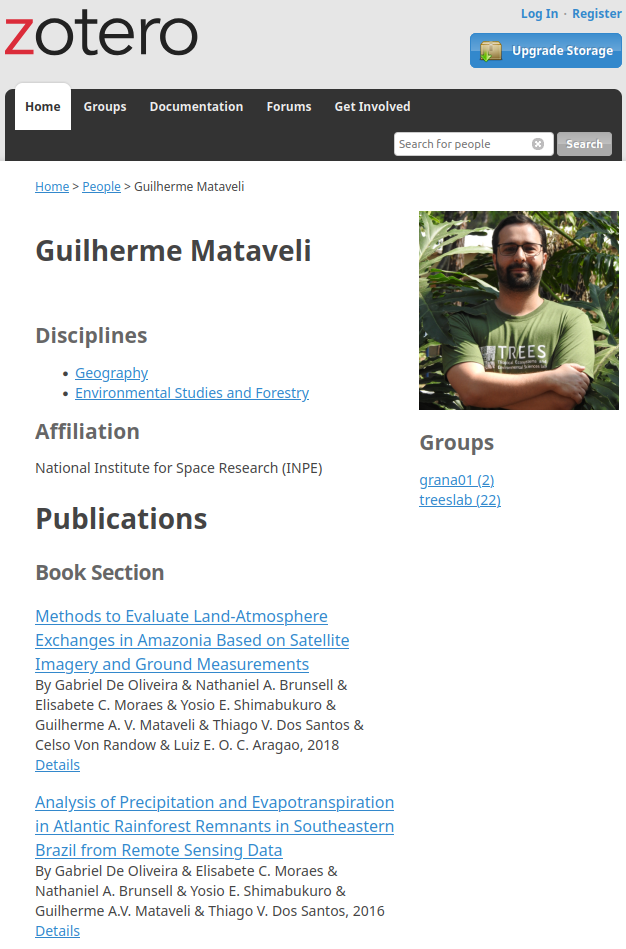
\includegraphics[scale=0.19]{images/zotero_guilherme_mataveli.png}
        \caption{A researcher's profile. Source:
        \href{https://www.zotero.org/gmataveli}{zotero.org}.}
      \end{figure}
    \end{column}
  \end{columns}
\end{frame}

\begin{frame}
  \begin{figure}
    \centering
    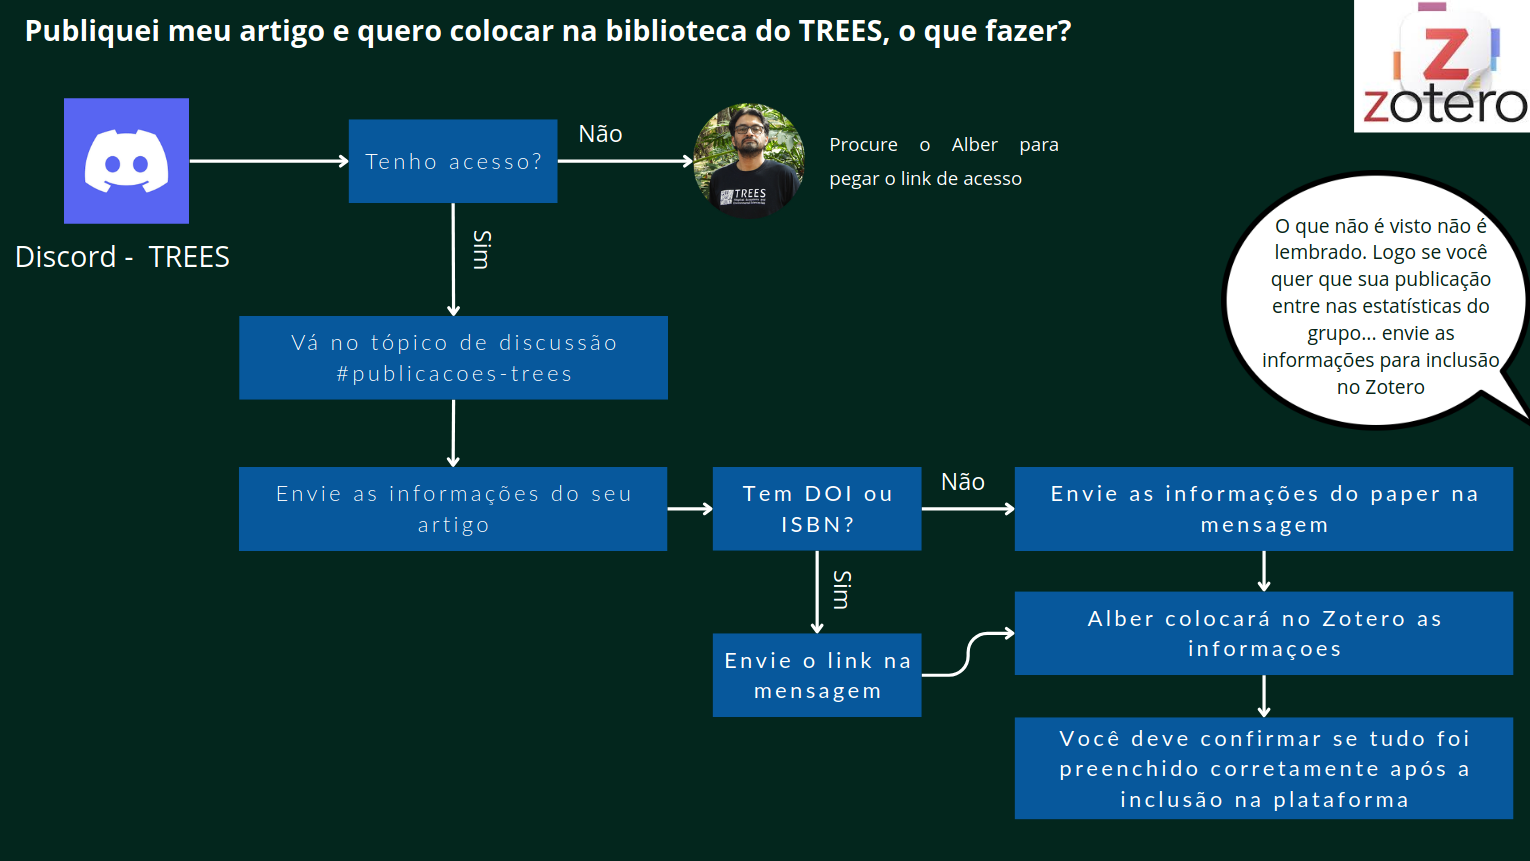
\includegraphics[scale=0.275]{images/zotero_treeslab_add.png}
  \end{figure}
\end{frame}

\begin{frame}
  \frametitle{Questions}
  \begin{itemize}
    \item \textit{Dificuldade de personalizar referências}
      \begin{itemize}
        \item Check slide~\ref{convert_styles}. \end{itemize}
    \item \textit{Como vincular ao Google Docs }
      \begin{itemize}
        \item Check slide~\ref{google_docs_zotero}.
      \end{itemize}
    \item \textit{Qual a vantagem do Zotero em relação ao Mendeley?}
      \begin{itemize}
        \item Check slide~\ref{tools-reference-management}.
      \end{itemize}
  \end{itemize}
\end{frame}

\section{Research data management}

\begin{frame}
  Research data management.
\end{frame}

\begin{frame}
  What do researchers do with the data associated to their publications?
\end{frame}

\subsection{Zenodo}

\begin{frame}
  \frametitle{Zenodo}
  \begin{columns}
    \begin{column}{0.5\textwidth}
      \begin{itemize}
        \item Open repository launched in 2013 and run by
          \href{https://home.cern/}{CERN}.
        \item Let researchers upload files up to 50 GB.
        \item It assigns a DOI to uploaded datasets.
        \item It supports GitHub repositories.
        \item It was named after Zenodotus, the first librarian of the Library
          of Alexandria~\cite{zenodo2013}.
      \end{itemize}
    \end{column}
    \begin{column}{0.5\textwidth}
      \begin{figure}
        \centering
        
\includegraphics[scale=0.07]{logos/zenodo-gradient-2500.png}
      \end{figure}
    \end{column}
  \end{columns}
\end{frame}

\begin{frame}
  \frametitle{Why use Zenodo?}
  Data could be lost due to many reasons:
  \begin{figure}
    \centering
    \begin{subfigure}[b]{0.3\textwidth}
      \centering
      
\includegraphics[width=\textwidth]{images/lost_laptop.png}
      \caption{Carelessness.}
    \end{subfigure}
    \hfill
    \begin{subfigure}[b]{0.3\textwidth}
      \centering
      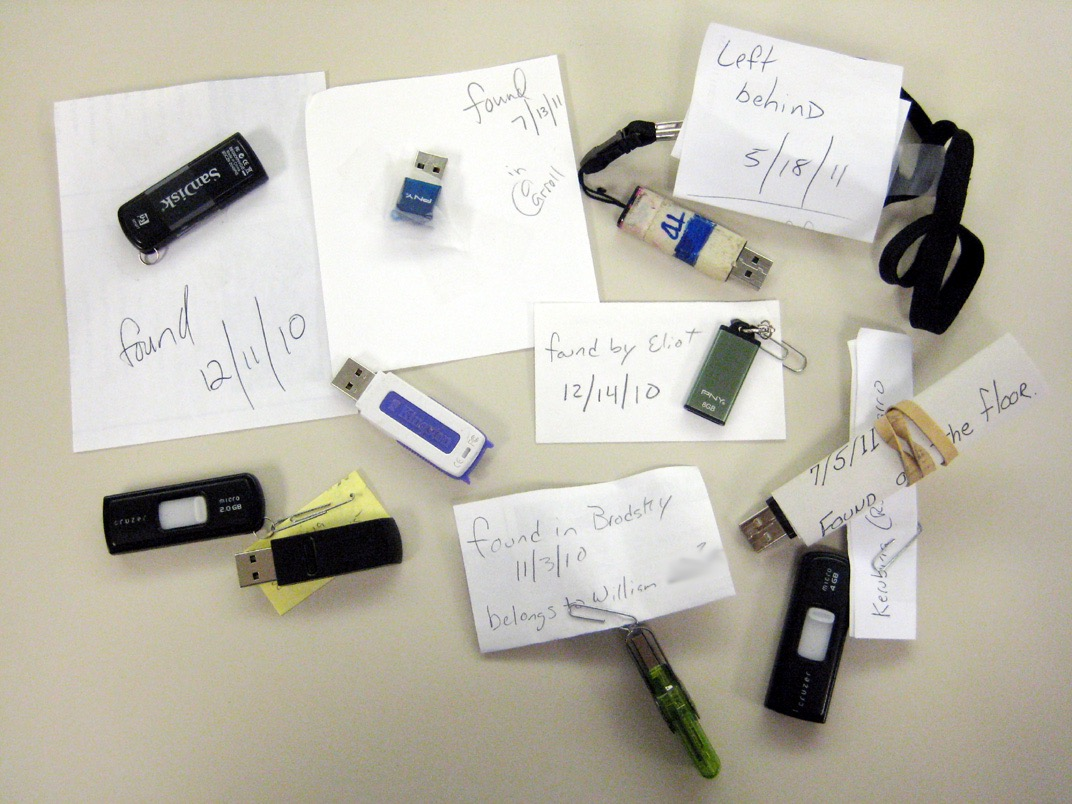
\includegraphics[width=\textwidth]{images/lost_usb_stick.png}
      \caption{Handling.}
    \end{subfigure}
    \hfill
    \begin{subfigure}[b]{0.3\textwidth}
      \centering
      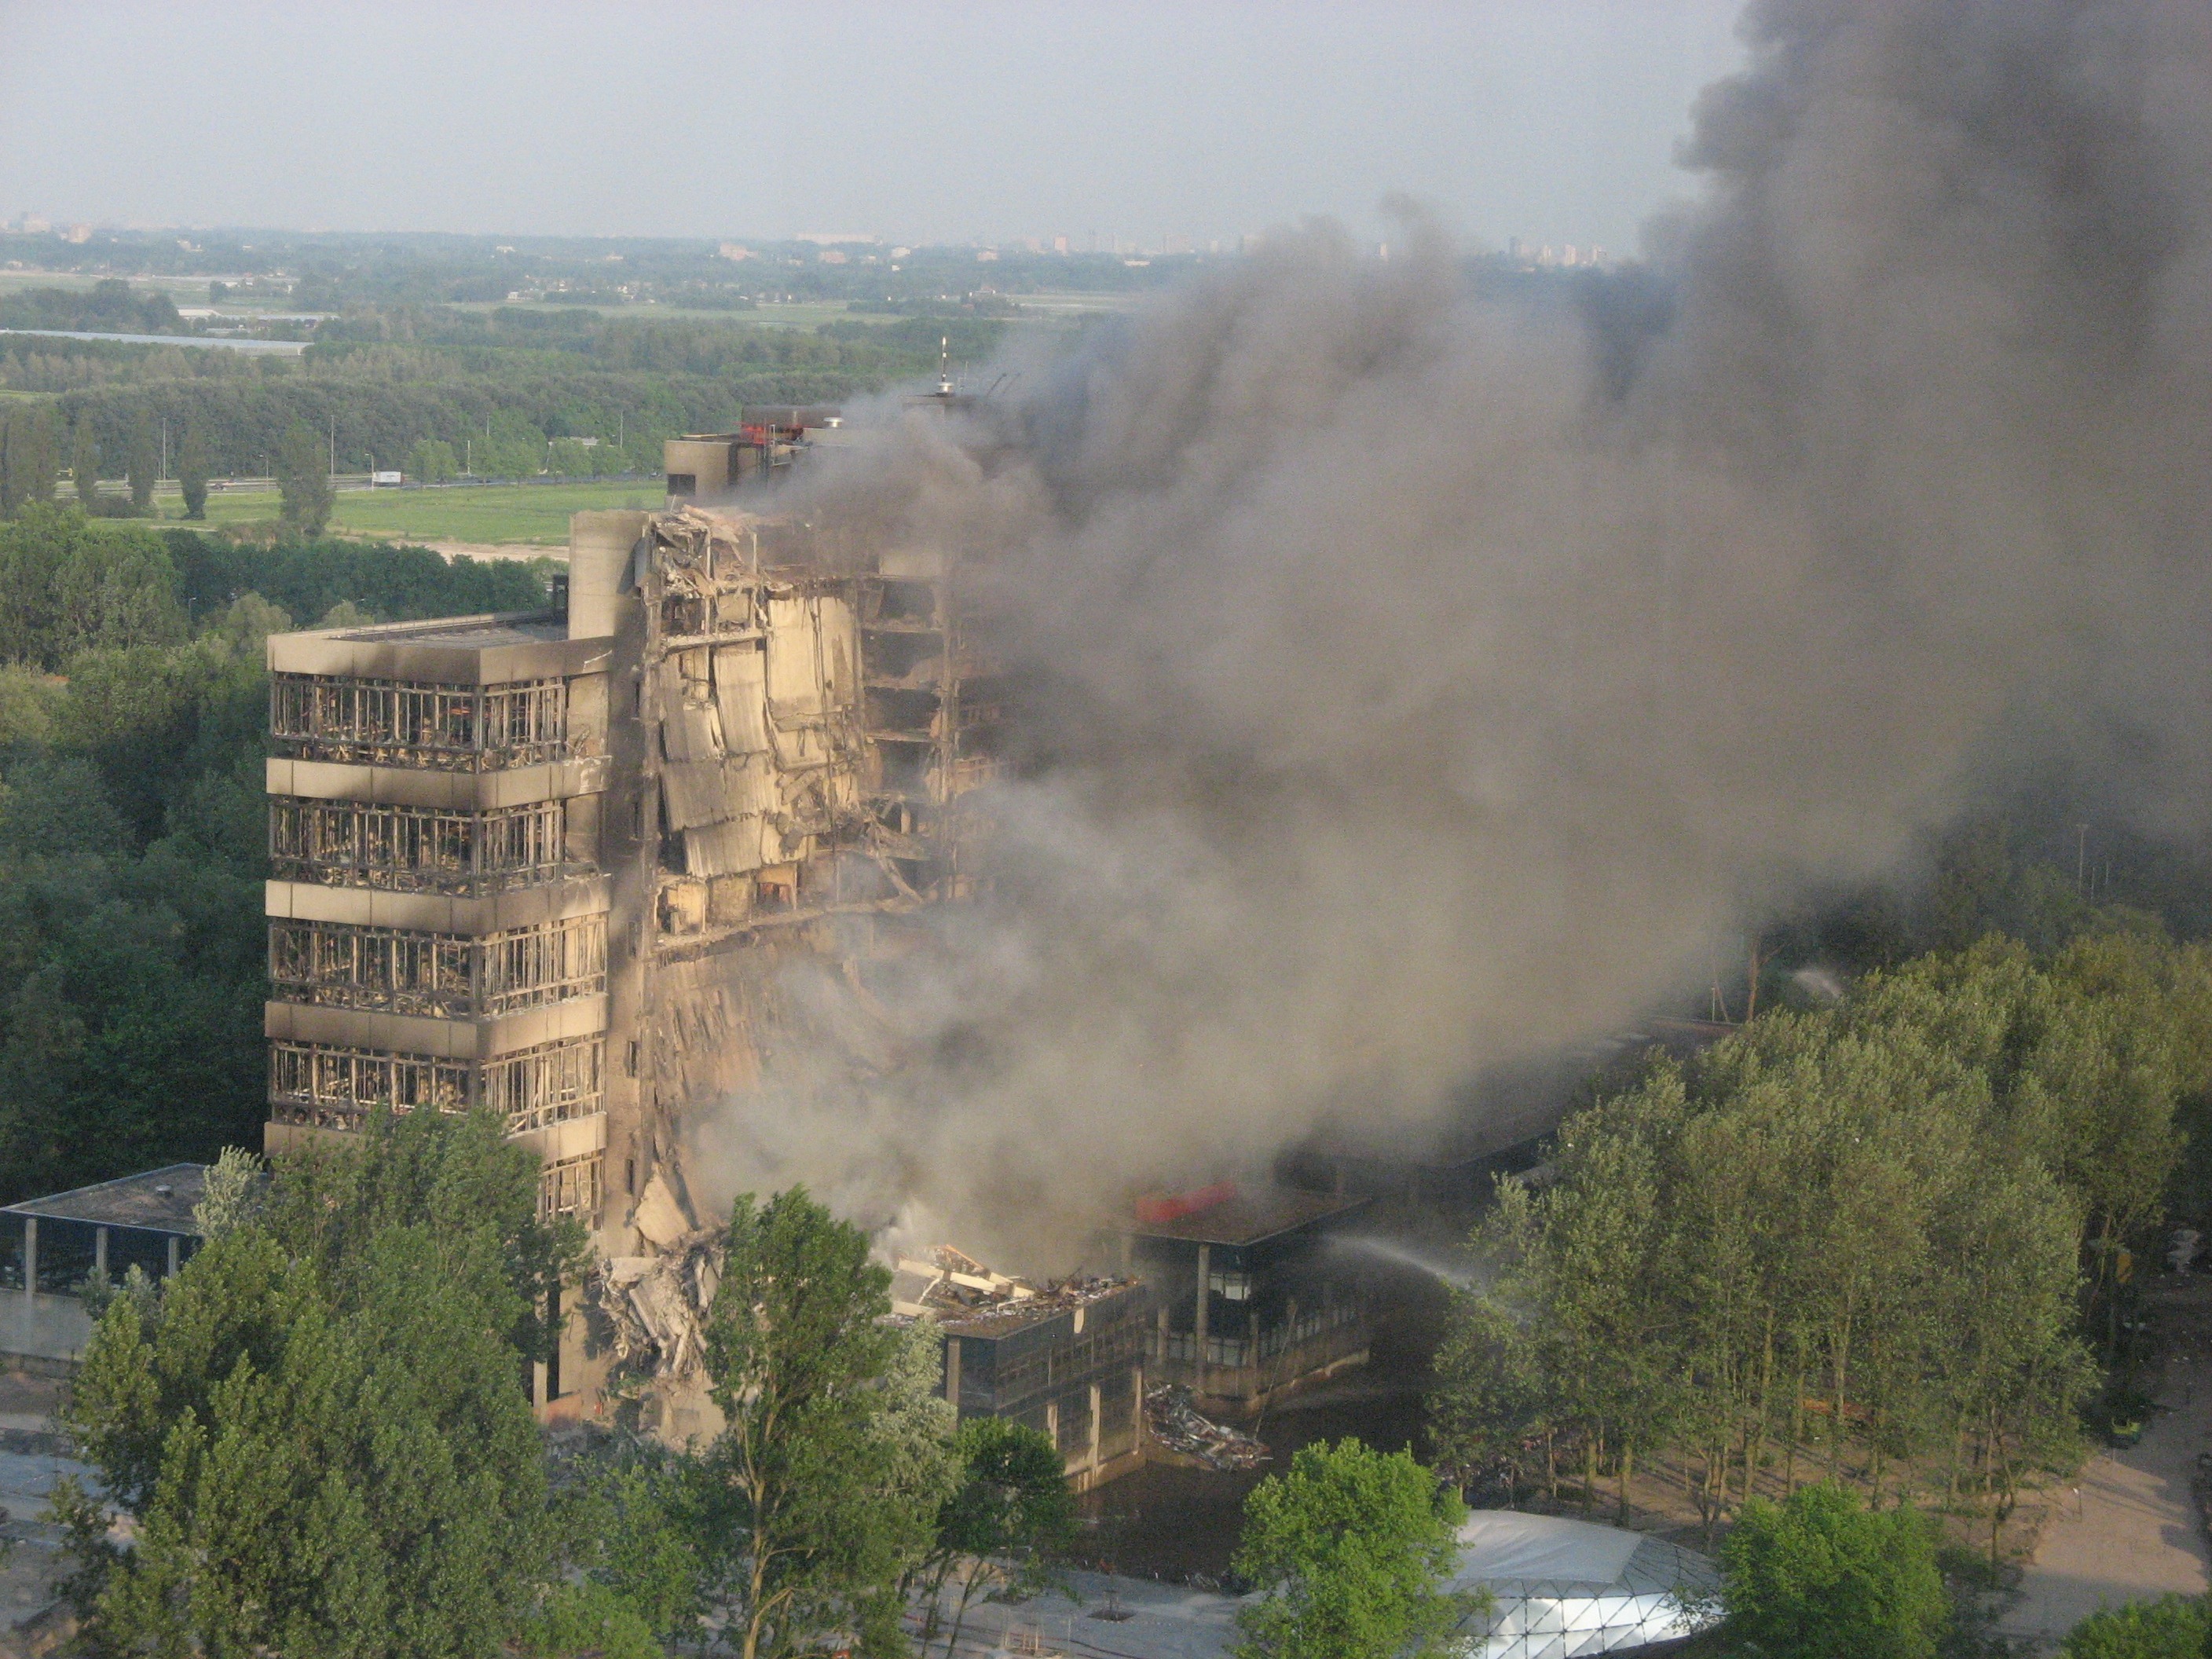
\includegraphics[width=\textwidth]{images/lost_building.png}
      \caption{Catastrophe.}
    \end{subfigure}
    \caption{Examples of data loss~\cite{nielsen2017}.}
  \end{figure}
\end{frame}

\begin{frame}
  \frametitle{Why use Zenodo?}
  \begin{columns}
    \begin{column}{0.5\textwidth}
      \begin{itemize}
        \item \textbf{Safe}: Data stored at CERN's data centre.
        \item \textbf{Trusted}: Operated by CERN.
        \item \textbf{No waiting time}: Available as soon as published.
        \item \textbf{Open or closed}: Restricted access mode.
        \item \textbf{Usage statistics}.
        \item \textbf{Versioning}: Update data and version numbers.
        \item \textbf{GitHub integration}: Preserve code.
        \item \textbf{Citeable}: Every upload has a DOI.
        \item \textbf{Data principles}: Findable, Accessible, Interoperable, Reusable.
      \end{itemize}
    \end{column}
    \begin{column}{0.5\textwidth}
      \begin{figure}
        \centering
        \includegraphics[scale=0.035]{logos/CERN-logo.png}
        
\includegraphics[scale=0.025]{logos/GitHub-Logo.png}
      \end{figure}
    \end{column}
  \end{columns}
\end{frame}

\begin{frame}
  \frametitle{Research data life cycle}
  \begin{figure}
    \centering
    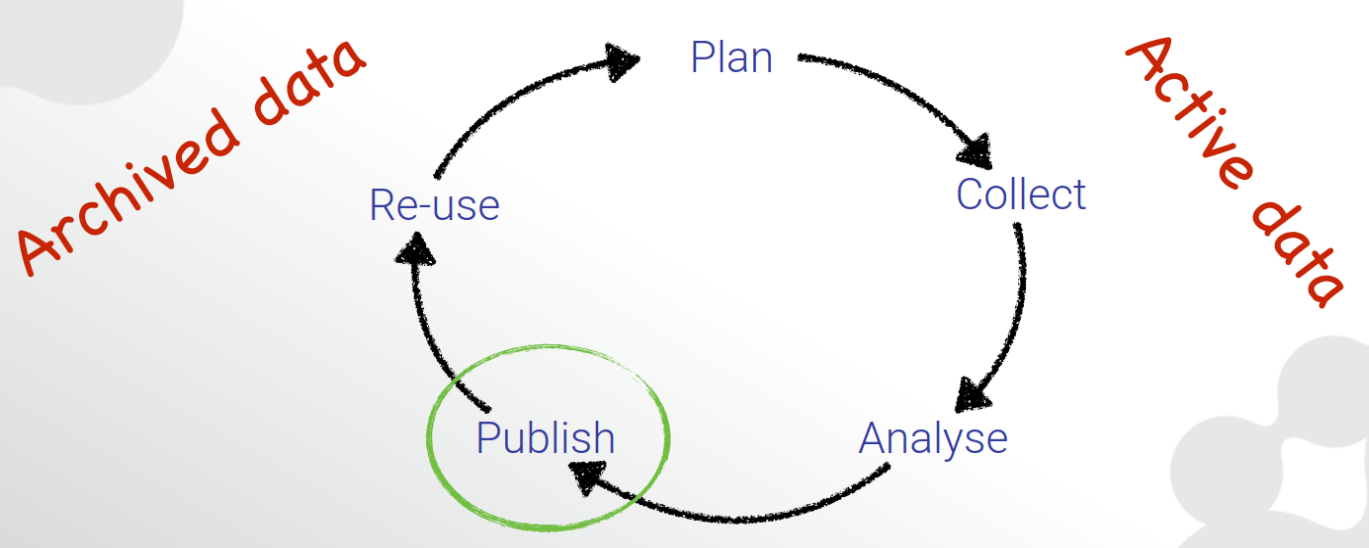
\includegraphics[scale=0.3]{images/zenodo_research_data_lifecycle.png}
    \caption{Research data life cycle according to
    ~\citeauthor{nielsen2017}~\cite{nielsen2017}.}
  \end{figure}
\end{frame}

\begin{frame}
  \frametitle{How do you do it?}
  \begin{columns}
    \begin{column}{0.5\textwidth}
      Sharing your data and software on Zenodo in 3
      steps~\cite{nielsen2017}:
      \begin{enumerate}
        \item Upload.
        \item Describe.
        \item Publish.
      \end{enumerate}
      By the way, the documents cited here, are themselves hosted at Zenodo!
    \end{column}
    \begin{column}{0.5\textwidth}
      \begin{figure}
        \centering
        
\includegraphics[scale=0.15]{images/zenodo_upload_describe_publish.png}
        \caption{Source: Poster presented in Dublin~\cite{nielsen2014}.}
      \end{figure}
    \end{column}
  \end{columns}
\end{frame}

\begin{frame}
  \frametitle{Upload}
  \begin{columns}
    \begin{column}{0.5\textwidth}
      Before you upload, think about:
      \begin{itemize}
        \item Data management plan.
        \item File formats (open versus proprietary).
        \item Standards.
        \item Re-usability.
        \item Licenses.
        \item Privacy.
      \end{itemize}
    \end{column}
    \begin{column}{0.5\textwidth}
      Zenodo allows:
      \begin{itemize}
        \item Any format.
        \item Any licence.
        \item Maximum of 50GB* and 100 files per dataset.
        \item Drag and drop upload.
      \end{itemize}
    \end{column}
  \end{columns}
\end{frame}

\begin{frame}
  \frametitle{Describe}
  \begin{columns}
    \begin{column}{0.5\textwidth}
      Basic information:
      \begin{itemize}
        \item Community (e.g. \textit{treeslab}).
        \item Authors or creators.
        \item Type: Dataset, image, model, poster, presentation, publication
          (book, chapter, conference paper or proceeding, report), software
          (notebook), video, audio.
        \item Title.
        \item Licenses.
      \end{itemize}
    \end{column}
    \begin{column}{0.5\textwidth}
      Recommended information:
      \begin{itemize}
        \item Contributors.
        \item Keywords and subjects.
        \item Dates.
        \item Version.
        \item Publisher.
      \end{itemize}
      Other information:
      \begin{itemize}
        \item Funding, alternate identifiers, related works, references,
          software, publishing information, conference, domain specific fields,
          visibility (public or restricted-embargo).
      \end{itemize}
    \end{column}
  \end{columns}
\end{frame}

\begin{frame}
  \frametitle{Publish}
  \begin{itemize}
    \item Files are not editable.
    \item Metadata is editable.
  \end{itemize}
\end{frame}

\subsection{Zenodo and TREESLab}

\begin{frame}
  \frametitle{TREESLab community at Zenodo}
  \begin{columns}
    \begin{column}{0.5\textwidth}
      \begin{itemize}
        \item You can publish any data to your Zenodo account.
        \item But you can also submit your data to the
          \href{https://tinyurl.com/treeslab-zenodo}{TREES' community}.
        \item This community accepts datasets related to publications produced
          by the TREES lab.
        \item Submissions are reviewed for quality and compliance to TREES
          standards.
      \end{itemize}
    \end{column}
    \begin{column}{0.5\textwidth}
      \centering
      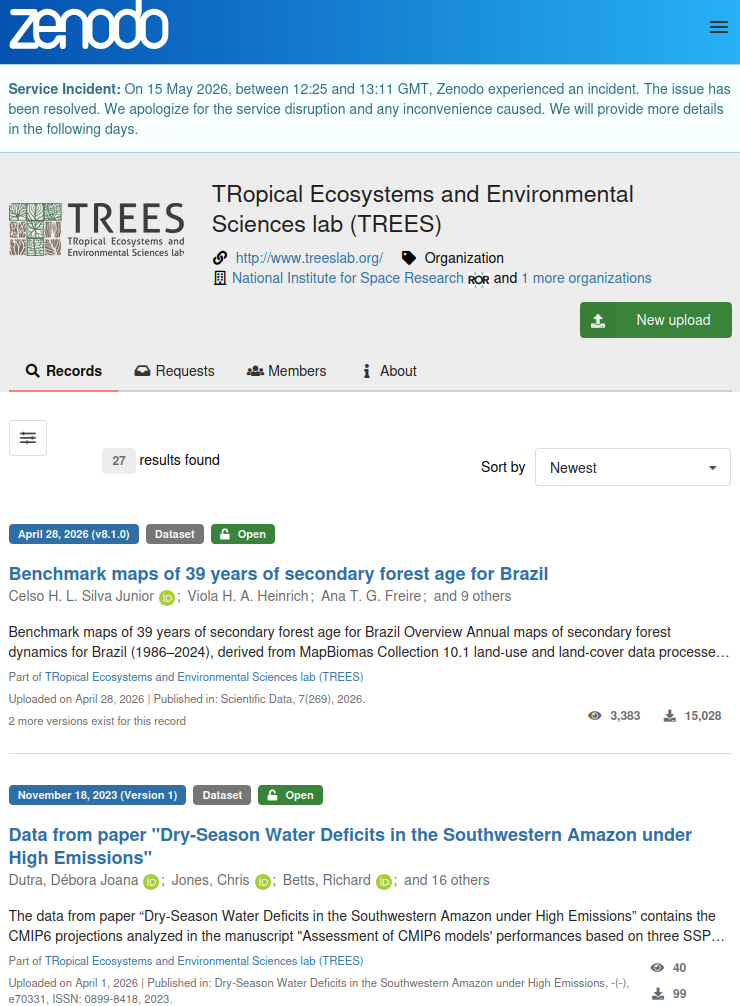
\includegraphics[scale=0.2]{images/zenodo_community_treeslab.png}
    \end{column}
  \end{columns}
\end{frame}

\begin{frame}
  \begin{figure}
    \centering
    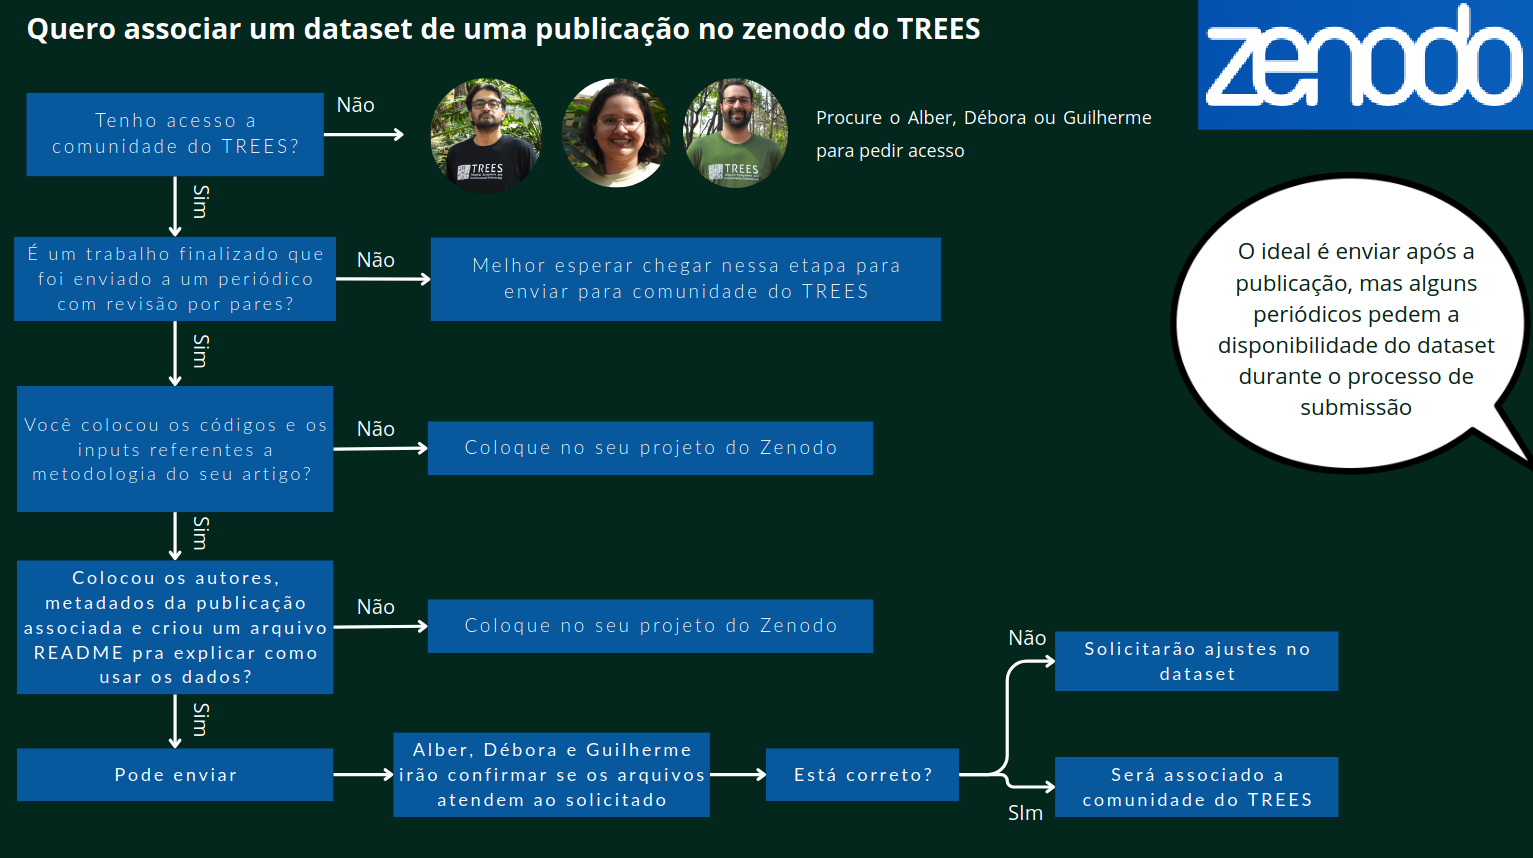
\includegraphics[scale=0.275]{images/zenodo_treeslab_add.png}
  \end{figure}
\end{frame}

\begin{frame}
  \frametitle{TREES' check list for Zenodo}
  \begin{columns}
    \begin{column}{0.5\textwidth}
      \begin{itemize}
        \item You \textbf{must} have an Zenodo account associated to TREES'
          community to submit datasets to this community.
        \item Your submission would be peer rewiewed by TREES' members (A + R
          in the \href{https://tinyurl.com/treeslab-membros}{RACI matrix}).
        \item To avoid common pitalls, we prepared a 
          (\href{https://docs.google.com/document/d/18ZKzcsP6GazzO0X5FDE8FUfkehaD3X3hoxrnWLSxI8o/edit?usp=sharing}
          {check list}).
        \item Read the check list before submitting your dataset to the TREES'
          community at Zenodo.
      \end{itemize}
    \end{column}
    \begin{column}{0.5\textwidth}
       Common recommendations include:
      \begin{itemize}
        \item Add a README.pdf file, describing the files in your submission.
        \item Your submission's name \textbf{must} start with
          \textit{"Data from ..."} or \textit{"Code for ..."}.
        \item Include the name of financing agencies (e.g. FAPESP, CAPES,
          CNPq).
        \item Fill in ZENODO's metadata fields: description, keywords, license,
          link to a publication.
      \end{itemize}
    \end{column}
  \end{columns}
\end{frame}

\begin{frame}
  Questions
  \begin{itemize}
    \item \textit{Qual o formato padrão proposto pelo Trees para o Zenodo.}
    \item \textit{Uma noção básica do funcionamento da plataforma.}
  \end{itemize}
\end{frame}

\section{Final remarks}

\begin{frame}
  Final remarks.
\end{frame}

\begin{frame}
  \frametitle{Final remarks}
  \begin{itemize}
    \item Please wonder if it is worth it to learn these tools, especially if
      you are going to be doing science \textbf{for the rest of your life}.
    \item Check
      \href{https://sites.unipampa.edu.br/sisbi/files/2023/08/manualzotero_versoafinal.pdf}
      {here} the \textit{Tutorial para gerenciamento de referências
      bibliográficas utilizando o software Zotero} by the Ibict.
    \item There is a check list for submissions to TREESLab's Zenodo community
      (check it \href{https://docs.google.com/document/d/18ZKzcsP6GazzO0X5FDE8FUfkehaD3X3hoxrnWLSxI8o/edit?usp=sharing}
          {here}).
    \item Also, check TREESLab' Discord chanels:
    \begin{itemize}
      \item \href{https://discord.com/channels/1207666629454856192/1215297398343999619}
      {ajuda-zotero}.
      \item \href{https://discord.com/channels/1207666629454856192/1215297581437947984}
        {ajuda-zenodo}.
    \end{itemize}
  \end{itemize}
\end{frame}

\begin{frame}
  \frametitle{RTFM}
  \begin{columns}
    \begin{column}{0.5\textwidth}
      \begin{itemize}
        \item Users don't acknowledge RTFM as their first option to solve
        software problems.
        \item This is so common, that software developers created RTFM as a
        gentle reminder to users of their options when dealing with software
        they don't know (check Wikipedia's article
        \href{https://en.wikipedia.org/wiki/RTFM}{about it}).
      \end{itemize}
    \end{column}
    \begin{column}{0.5\textwidth}
      \begin{figure}
        \centering
        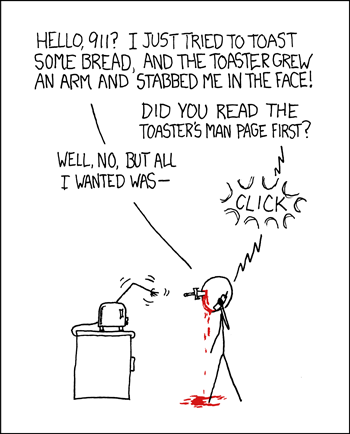
\includegraphics[scale=0.4]{images/rtfm.png}
        \caption{Source: RTFM by \href{https://imgs.xkcd.com/comics/rtfm.png}{xkcd}.}
      \end{figure}
    \end{column}
  \end{columns}
\end{frame}


\section{References}

\begin{frame}
  References
\end{frame}

\begin{frame}[allowframebreaks]
  \printbibliography
\end{frame}

\end{document}
